\section{Results}

The code for analog simulation is listed in \cref{app:analog}. 
Code for digital control logic is listed in \cref{app:digital}. 
All the plots were created with the MATLAB code in \cref{app:other:matlab}.

\subsection{Analog}
\label{Analog_res}
The analog readout circuit was simulated thoroughly with different exposure voltages to simulate multiple lighting conditions. 
In \cref{fig:res:anal:all@2ms} the simulation result at 2ms exposure time is presented. 
In the first and second plot pane the erase and exposure voltages are presented. 
Both of these voltages influence the sampled voltages which are presented in the third plot pane. 
This plot pane shows the behaviour of the capacitor at different photodiode currents 200pA, 250pA, 500pA and 750pA.
The Fourth plot pane shows the read enable transistor voltages in the same simulation. 
These are active low, meaning that they will have a voltage drop when activated. 
The final plot plane shows the circuit output voltages, which are thought to be sent to an ADC.

\begin{figure}[!htbp]
    \centering
    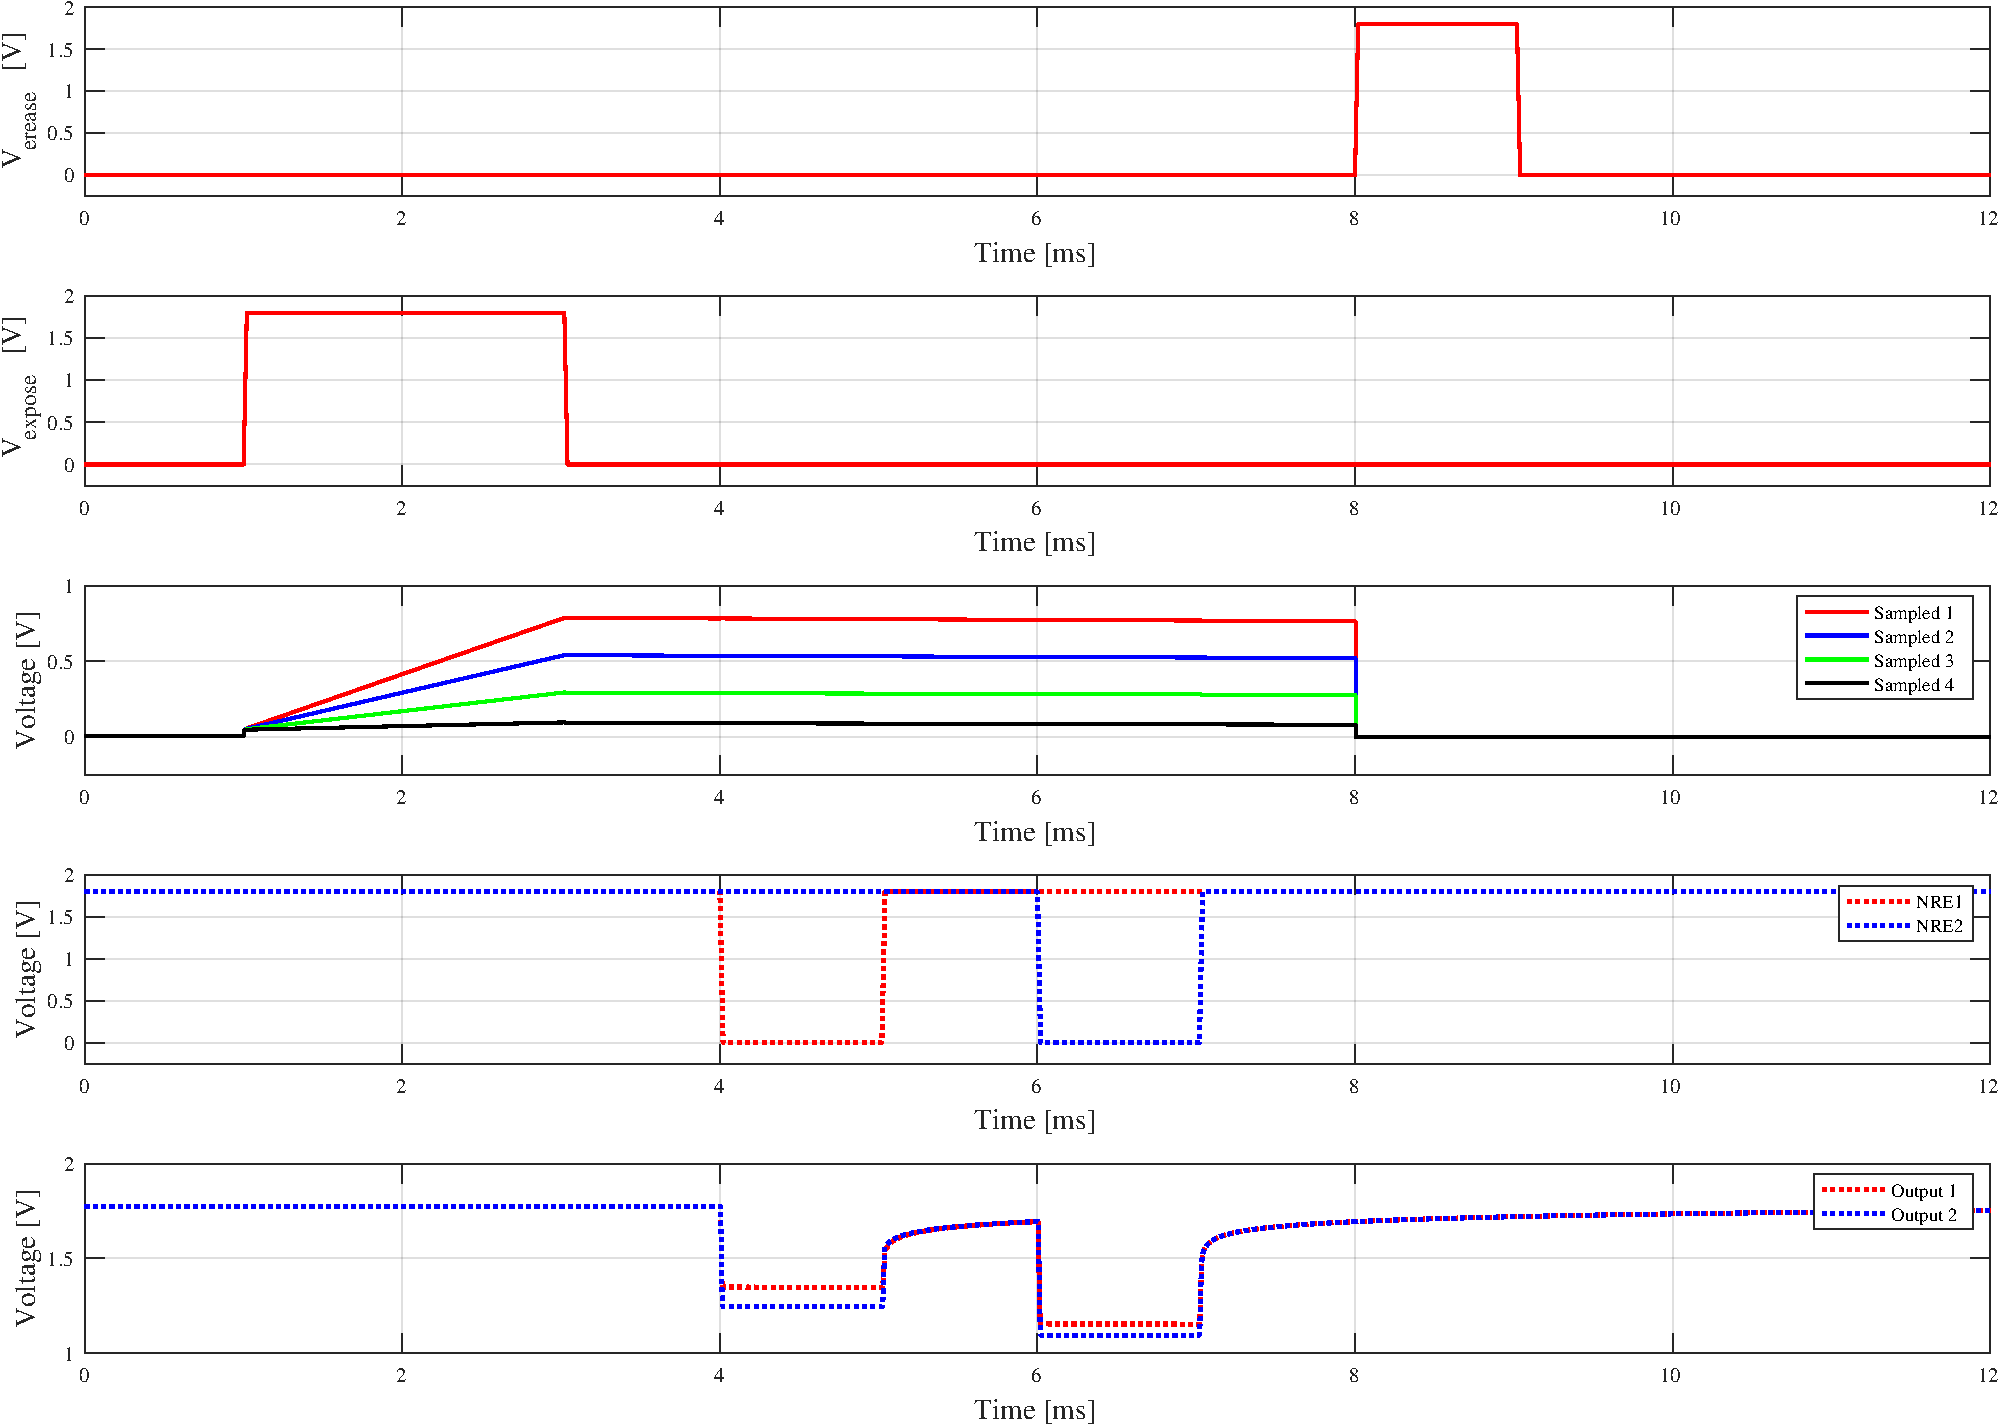
\includegraphics[width=\textwidth]{Images/Analog_plots/all_in_1.pdf}
    \caption{Node voltages at 2ms exposure time, under different photodiode currents}
    \label{fig:res:anal:all@2ms}
\end{figure}

The same node-voltages are simulated and plotted in \cref{fig:res:anal:all@30ms} at a longer exposure time of 30ms, where it shows that the lower photo diode currents will saturate the capacitor. 
The same photo diode currents as before are simulated here i.e. 200pA, 250pA, 500pA and 750pA.

\begin{figure}[H]
    \centering
    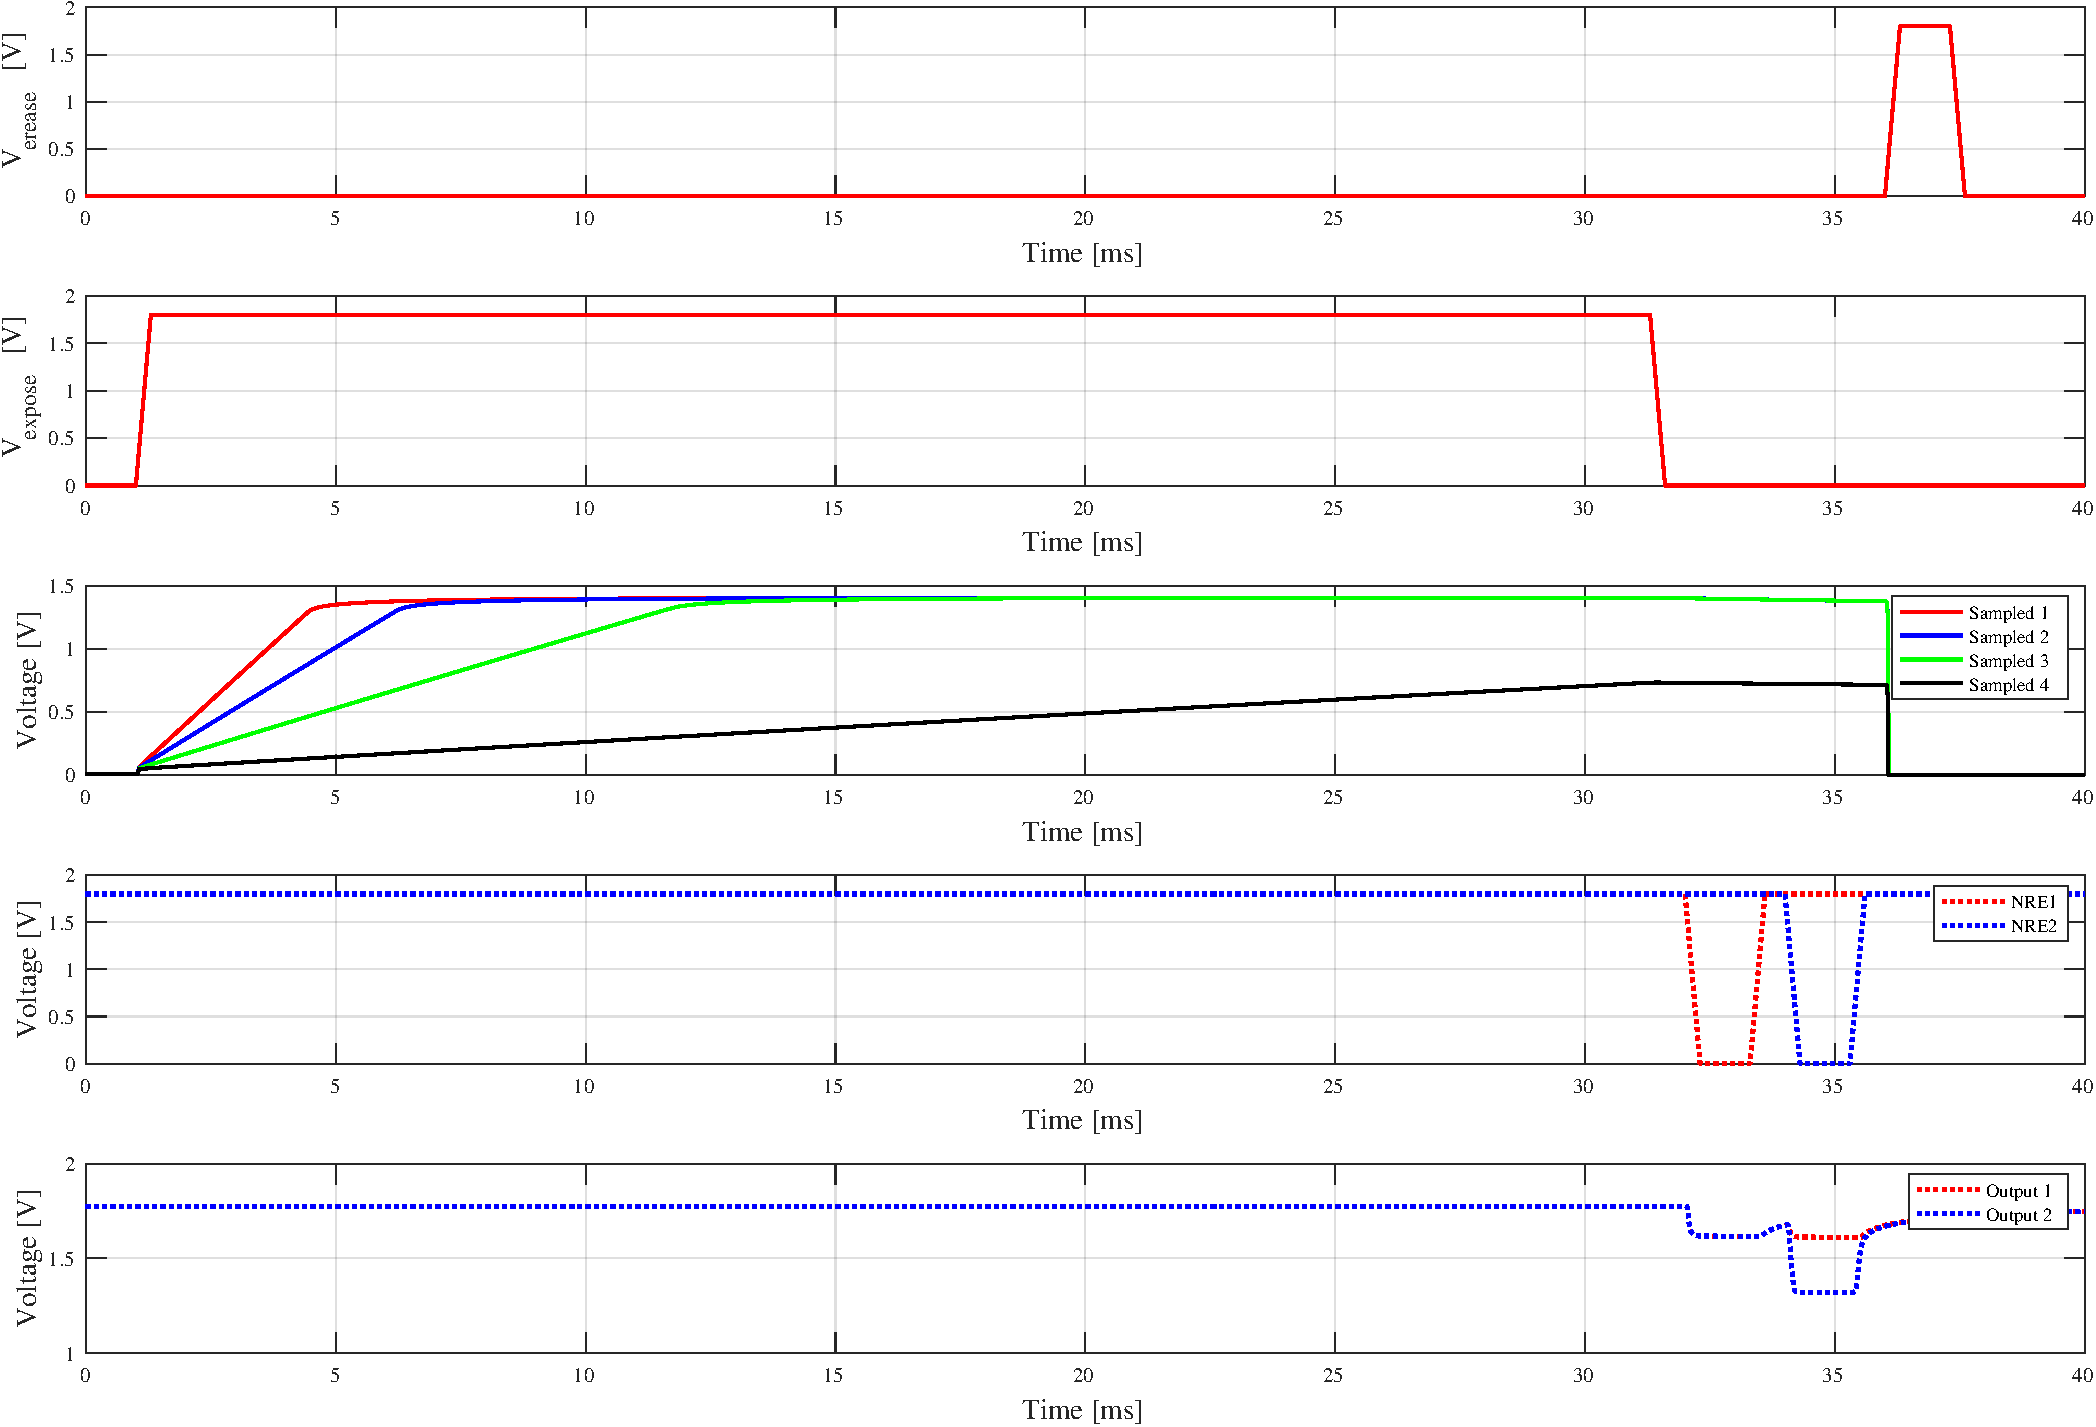
\includegraphics[width=\textwidth]{Images/Analog_plots/all_in_1@30ms.pdf}
    \caption{Node voltages at 30ms exposure time, under different photodiode currents}
    \label{fig:res:anal:all@30ms}
\end{figure}

\Cref{fig:res:anal:all2} shows the same simulation as \cref{fig:res:anal:all@2ms}, but a closer look at the capacitor voltage response to the exposure voltage and erase voltage. 
It shows that the exposure voltage charges the capacitor up to a certain voltage potential, dependent on the diode current and exposure time. 
It also shows that when the erase transistor receives its voltage, the capacitor discharges, and is ready for a new exposure. 

\begin{figure}[H]
    \centering
    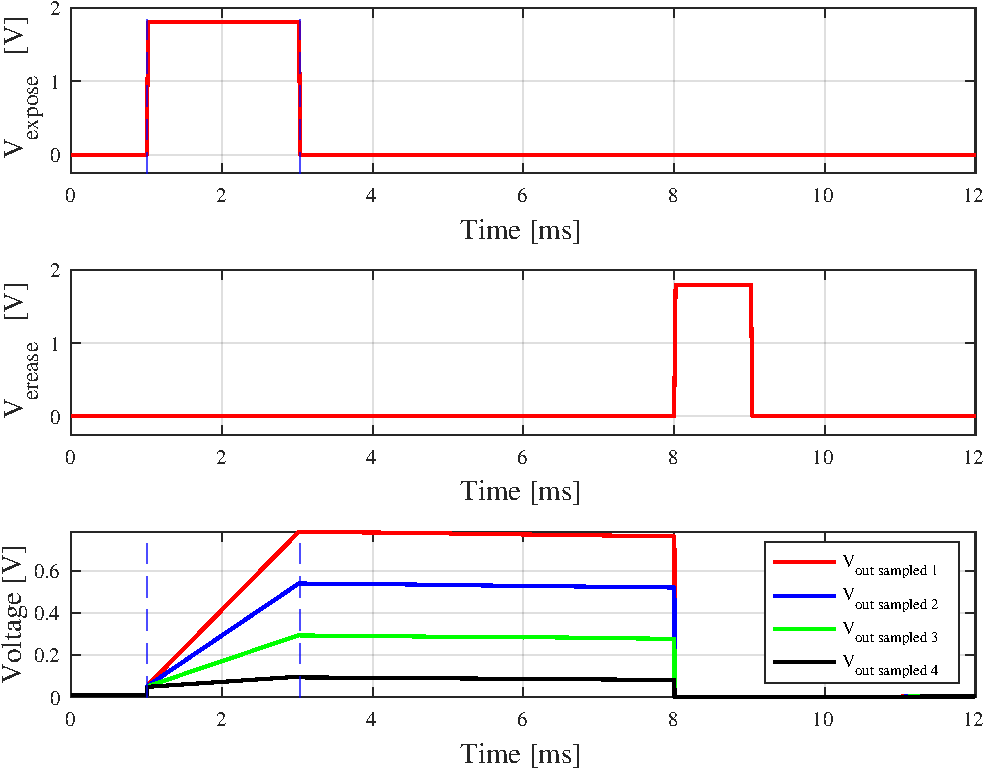
\includegraphics[width=\textwidth]{Images/Analog_plots/exp_eras_sample_m_voltage.pdf}
    \caption{Capacitor voltages vs. control voltages}
    \label{fig:res:anal:all2}
\end{figure}

\Cref{fig:res:anal:all3} shows a closer look at the capacitor voltages at 2ms exposure under the four different lighting conditions, i.e. diode currents.

\begin{figure}[H]
    \centering
    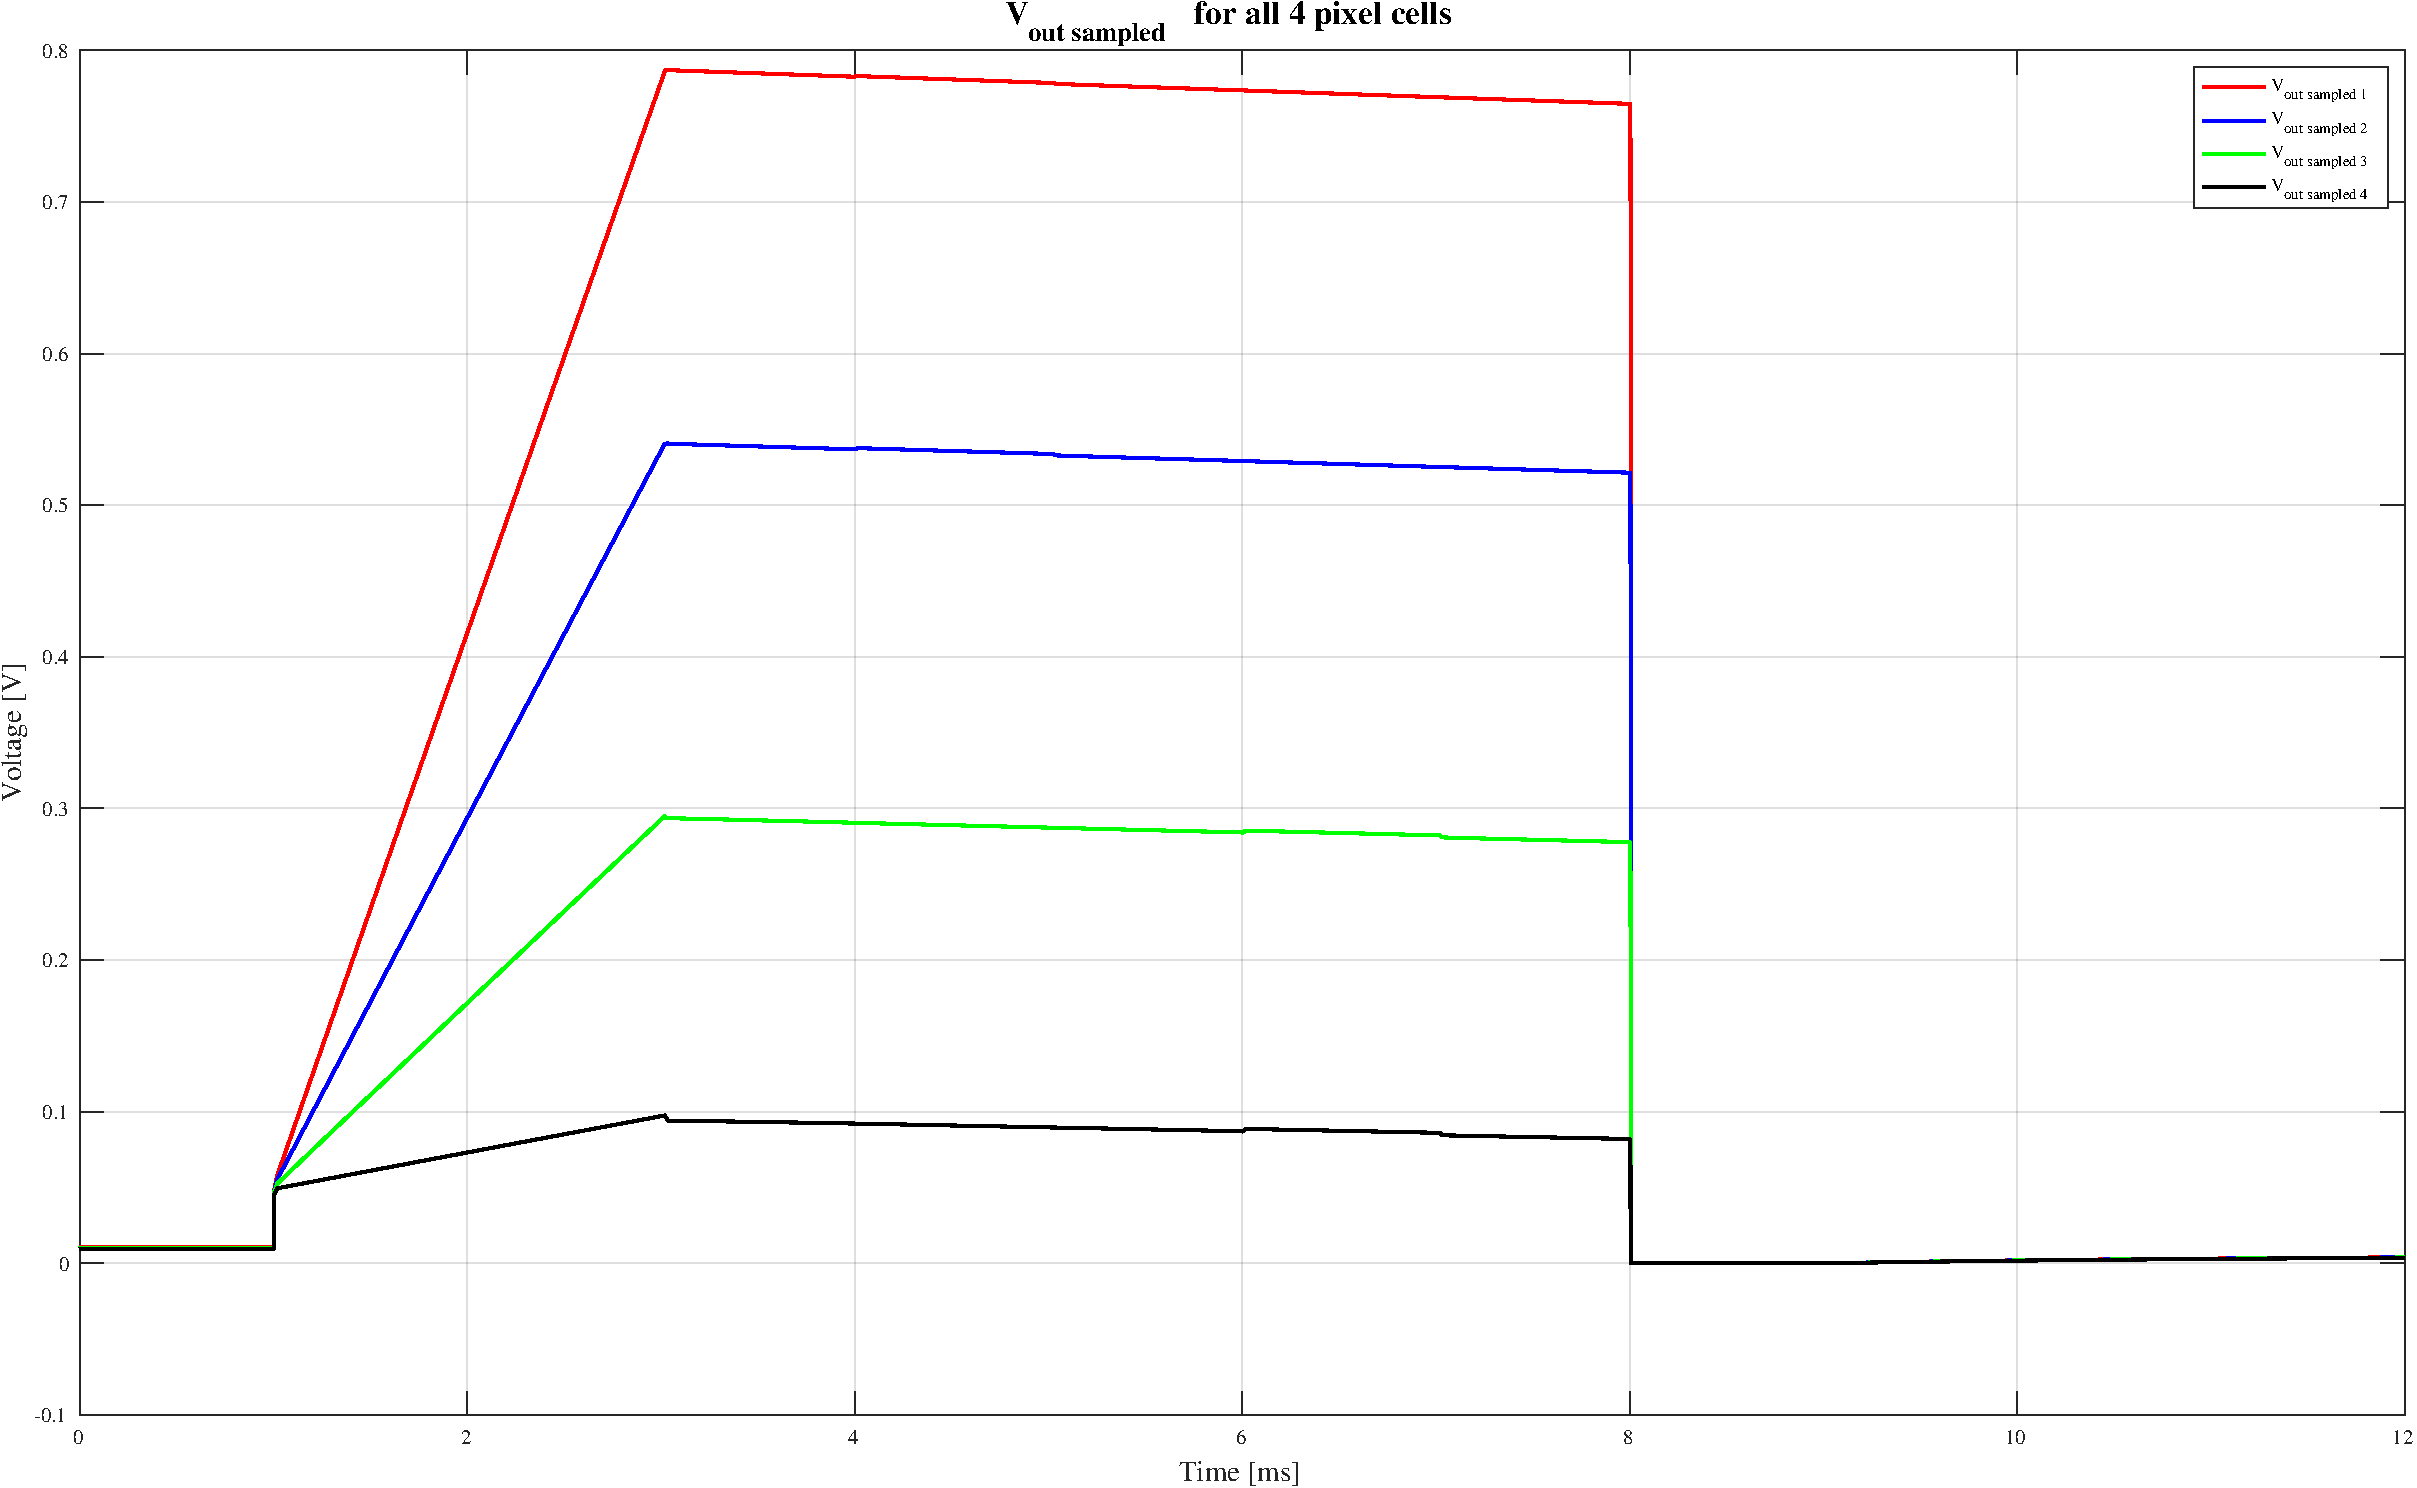
\includegraphics[width=\textwidth]{Images/Analog_plots/v_out_sampled_all_2ms.pdf}
    \caption{Capcitor voltages under different lighting conditions at 2ms exposure time}
    \label{fig:res:anal:all3}
\end{figure}


\subsubsection{Corner analysis}
As mentioned in \cref{Corn_analysis}, a corner analysis of an NMOS switch was done. 
The transconductance of an NMOS where plotted using three different process corners, TT, FF and SS. 
The SPICE net used for this simulation is included in \cref{app:switch}

\begin{figure}[H]
    \centering
    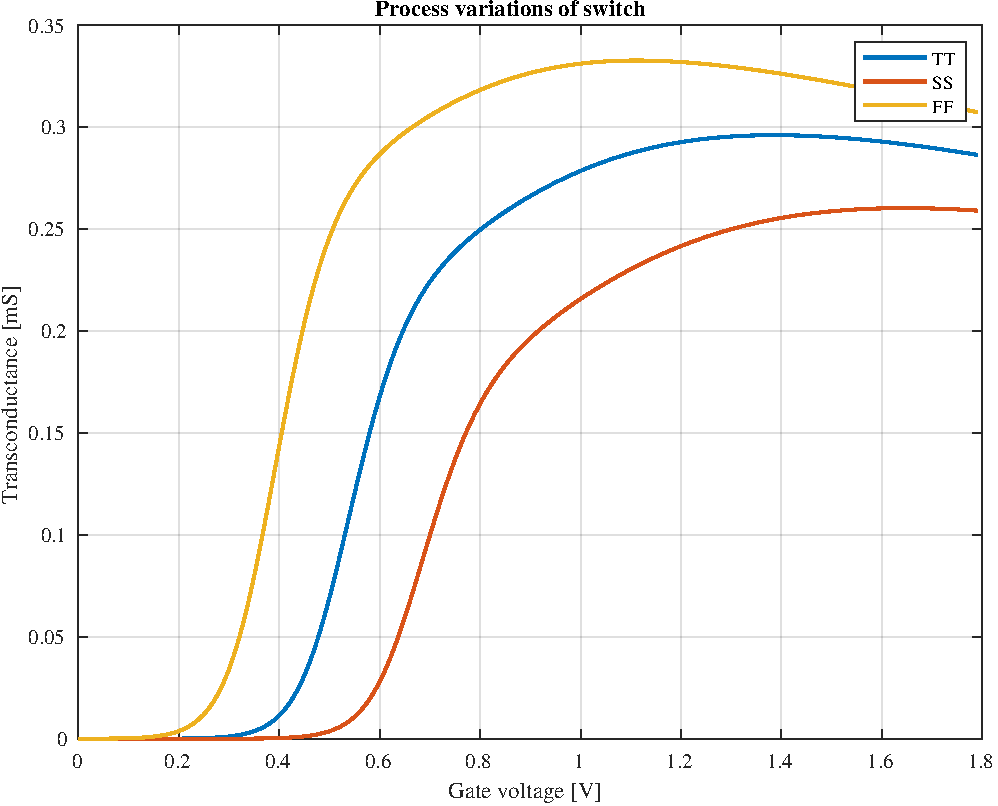
\includegraphics[width=\textwidth]{Images/Analog_plots/corneranalysis.pdf}
    \caption{Corner analysis of NMOS switch}
    \label{fig:res:anal:corn_nmos}
\end{figure}


\subsection{Digital}

All verilog code was compiled with Icarus Verilog \cite{williams_2020}, \mintinline{bash}{iverilog}. 
To compile with SystemVerilog 2005 use the flag \mintinline{bash}{-g2005-sv}.

\Cref{fig:res:dig:timer} shows the timing diagram for the \texttt{timer\_counter} block.
To set the initial value to count from, it is shown set the \texttt{ex\_set} high.
When \texttt{ex\_start} is set high the timer start counting down to $0$.
When it reaches $0$ the signal \texttt{ex\_done} is set high.

\begin{figure}[!htbp]
    \centering
    \fbox{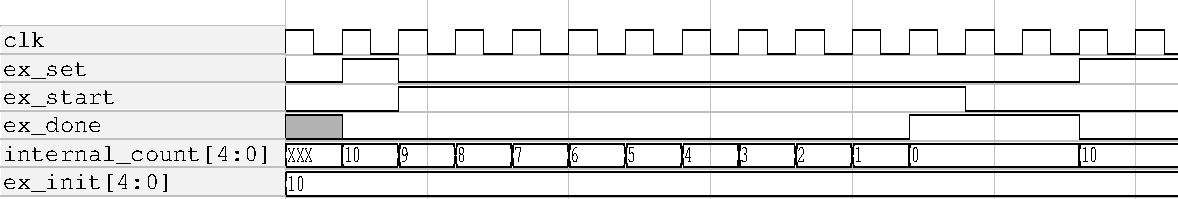
\includegraphics[width=.95\textwidth]{Images/Digital_plots/timer_counter_tb.pdf}}
    \caption{Timing diagram for the \texttt{timer\_counter} block. Larger version in \cref{app:figs:timer_counter}}
    \label{fig:res:dig:timer}
\end{figure}

\Cref{fig:res:dig:CTRL} shows the timing diagram for the \texttt{CTRL\_ex\_time} block.
When \texttt{ex\_increase} is set high, it will increase the exposure time by one for each clock cycle.
Similar for \texttt{ex\_decrease}, but it decreases the exposure time. 

There is a maximum and minimum value of 30 ms and 2 ms respectively. 
Both inc/decrease and the limits are tested and shown in \cref{fig:res:dig:CTRL}.
When \texttt{reset} is set high, the initial value is set to $16$, which is in the middle of $30$ and $2$.

\begin{figure}[!htbp]
    \centering
    \fbox{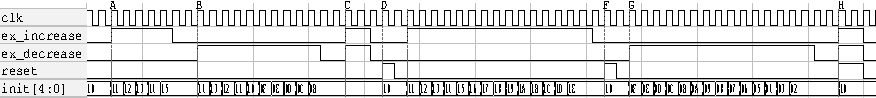
\includegraphics[width=.95\textwidth]{Images/Digital_plots/CTRL_ex_time_tb.pdf}}
    \caption{Timing diagram for the \texttt{CTRL\_ex\_time} block. Larger version in \cref{app:figs:CTRL}}
    \label{fig:res:dig:CTRL}
\end{figure}

In \cref{fig:res:dig:FSM}, the timing diagram for the main logic block, \texttt{FSM\_ex\_control}, is shown.
The FSM is reset when \texttt{reset} is high. This happens at \texttt{A}. At \texttt{B} we have a state change into EXPOSING. This is done until \texttt{ex\_done} is set high. 
When this happens at \texttt{C}, the state is set to READOUT, and the readout sequence for the pixel array is initiated. 
At \texttt{D} and \texttt{E} the FSM returns to the IDLE state, finishing the sequence of capturing a picture.

\begin{figure}[!htbp]
    \centering
    \fbox{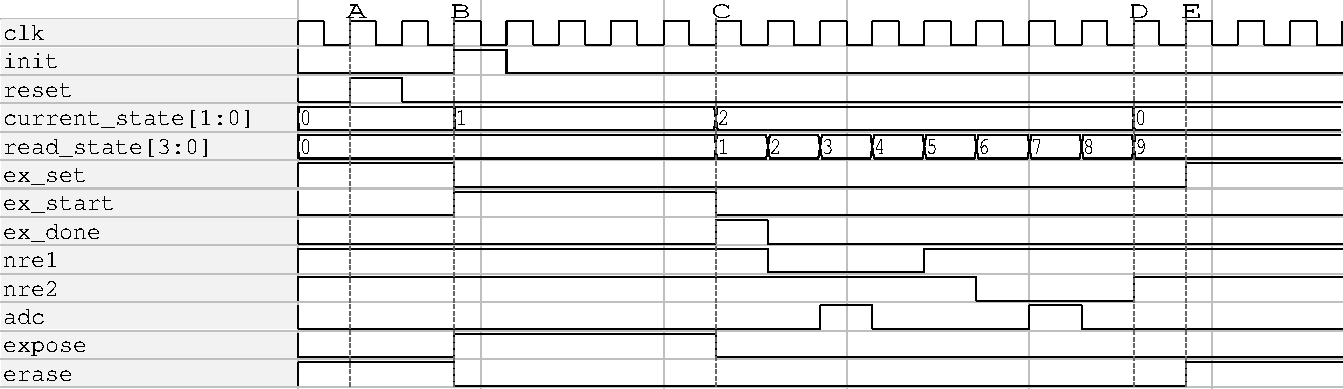
\includegraphics[width=.95\textwidth]{Images/Digital_plots/FSM_ex_control_tb.pdf}}
    \caption{Timing diagram for the \texttt{FSM\_ex\_control} block. Larger version in \cref{app:figs:FSM}}
    \label{fig:res:dig:FSM}
\end{figure}

\Cref{fig:res:dig:re_control} is the combined timing diagram for the top level block, \texttt{re\_control}. 
When resetting at \texttt{A}, we can continue by decreasing the exposure time at \texttt{B}.
This is done until we have 10 ms exposure. At \texttt{C}, we initiate the capture sequence by exposing and starting the exposure counter.
At \texttt{D} the exposure is done, 10 clock cycles later than initialization (at 1kHz that is 10ms).
Following is the readout, same as in \cref{fig:res:dig:FSM}. 
At \texttt{E} the sequence is done and all values are set back to the initial values and the state is set to IDLE.

\begin{figure}[!htbp]
    \centering
    \fbox{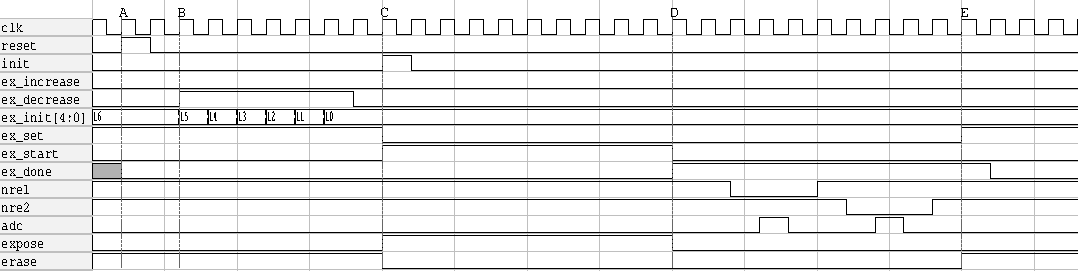
\includegraphics[width=.95\textwidth]{Images/Digital_plots/re_control_tb.pdf}}
    \caption{Timing diagram for the \texttt{re\_control} block. Larger version in \cref{app:figs:re_control}}
    \label{fig:res:dig:re_control}
\end{figure}